\documentclass[aspectratio=169, handout]{beamer}
%la opcion hangout es para complilar en modo imprimible
%\documentclass[hangout]{beamer}

\mode<presentation>
{
  \usetheme{Berkeley}
  \setbeamercovered{transparent}
  \setbeamertemplate{navigation symbols}{}
}

\usepackage[spanish]{babel}
\usepackage[utf8]{inputenc}
\usepackage{tikz}
\usepackage{textpos}
\usepackage{hyperref}
\usepackage{caption}
\captionsetup[figure]{labelformat=empty}

%\usetikzlibrary{shapes,arrows}
\setbeamerfont{author}{size=\large}
\setbeamerfont{institute}{size=\normalsize\bfseries}
\setbeamerfont{title}{size=\Large\bfseries}
\setbeamerfont{subtitle}{size=\huge}

\definecolor{darkblue}{RGB}{51,51,179}
\setbeamercolor{bgcolor}{fg=white,bg=darkblue}

\title[802.15.4 LR-WPAN]{Protocolos de Comunicación en Sistemas Embebidos}
\subtitle{Práctica 802.15.4 LR-WPAN}
\author[]{Ing. Patricio Bos, Esp. Ing. Juan Montilla}
\institute[CESE-FIUBA]{Carrera de Especialización en Sistemas Embebidos - FIUBA}
\date{}

%\subtitle{Framework para aplicaciones de control de ambientes}
\titlegraphic{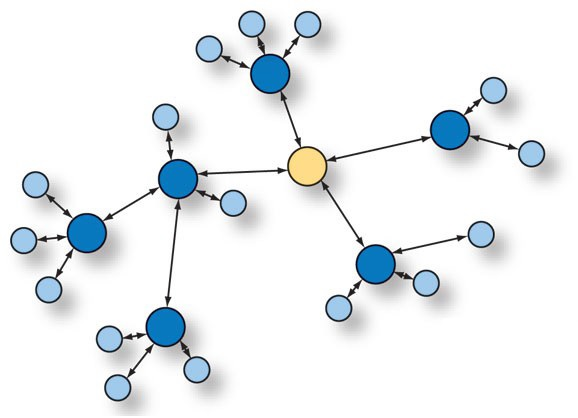
\includegraphics[width=5cm]{./imagenes/red.jpg}}


\subject{Protocolos y Comunicaciones: 802.15.4 LR-WPAN. Carrera de Especialización en Sistemas Embebidos}
% This is only inserted into the PDF information catalog. Can be left
% out. 

\pgfdeclareimage[height=1.5cm]{university-logo}{./imagenes/logo-facu-inverso.png}
\logo{\pgfuseimage{university-logo}}


% If you wish to uncover everything in a step-wise fashion, uncomment
% the following command: 

\beamerdefaultoverlayspecification{<+->}
  
\begin{document}

%Captions sin el texto "Figure"
\setbeamertemplate{caption}{\raggedright\insertcaption\par}

%la magia del begingroup es para que titlepage quede centrada, sin eso queda
%corrida en el ancho del sidebar
%\begingroup
%\makeatletter
%\setlength{\hoffset}{-.5\beamer@sidebarwidth}
%\makeatother
%\begin{frame}[plain,noframenumbering]
%  \titlepage
%\end{frame}
%
%\endgroup


%-------------------------------------------------%
%-------------------------------------------------%
% PORTADA
%-------------------------------------------------%
%-------------------------------------------------%

\begingroup
\makeatletter
\setlength{\hoffset}{-.5\beamer@sidebarwidth}
\makeatother
\begin{frame}[plain,noframenumbering]
\begin{center}
%\vspace{5px}
\hfill
    \begin{beamercolorbox}[center,dp=3ex,ht=10.25ex, wd=1\linewidth]{bgcolor}
        \Large\textbf{Protocolos de Comunicación en Sistemas Embebidos}\\
        \huge\textbf{Práctica 802.15.4 LR-WPAN}
    \end{beamercolorbox}
\hfill\hfill
\\
\vspace{5px}
\textbf{Carrera de Especialización en Sistemas Embebidos - FIUBA}\\
\vspace{10px}
\texttt{Ing. Patricio Bos}\\
\texttt{Esp. Ing. Juan Montilla}\\

\vspace{10px}

\begin{figure}[H]
	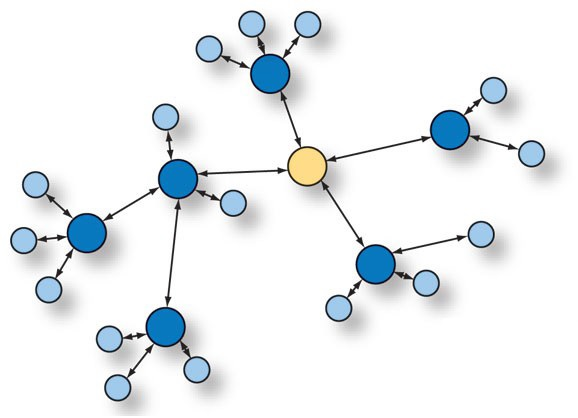
\includegraphics[width=.3\textwidth]{./imagenes/red.jpg}
\end{figure}	  	  	
\vspace{5px}
\tiny versión: 2016-06-06 rev 1.0 

\end{center}
\end{frame}
\endgroup

%-------------------------------------------------%
%-------------------------------------------------%

\begin{frame}{\textbf{Organización de la práctica}}
  \tableofcontents
  % You might wish to add the option [pausesections]
\end{frame}
%
%
%-------------------------------------------------%
\section[Herramientas]{Herramientas}
%-------------------------------------------------%
\begin{frame}[c]{Herramientas}
%\vspace{10px}
    \begin{itemize}

        \item Toolchain: LPCxpresso
            \begin{itemize}
            \item IDE basado en eclipse + compiler y linker GNU + GDB debugger.
            \vspace{10px}
            \item LPC-Link: Herramienta que incluye un programador y debugger.
            \vspace{10px}   
            \end{itemize}
        \item Target: LPC1343 ARM Cortex-M3 (Mote LSE).
        \vspace{10px}
    \end{itemize}
\end{frame}

%
%-------------------------------------------------%
%-------------------------------------------------%
\section{Práctica 802.15.4 LR-WPAN}
%-------------------------------------------------%
%-------------------------------------------------%

%-------------------------------------------------%
\subsection[Estrella]{Topología Estrella}
%-------------------------------------------------%

\begin{frame}[t]{Ejercicio 1: Topología Estrella}
%\vspace{10px}
\begin{columns}[t]
    \begin{column}{.5\textwidth}
        \begin{minipage}[t][0.7\textheight][s]{\columnwidth}
            \begin{itemize}
            \item Se dispone de una topología de tipo Estrella:
            \begin{itemize}
                \item Un Mote como coordinador.
                \item El resto como device.
            \end{itemize}
            \vspace{5px}
            \item Transferencia de datos:
            %\vspace{5px}
            \begin{itemize}
                \item Todas las tramas son de tipo Data.
                \item La inicia el device: Data request.
                \item Se debe enviar acuse de recibo por cada trama recibida.
                \item El coordinador envía una trama al device que lo solicite. El payload contiene el mensaje: "hola deviceN". Con N la respectiva dirección remota.
            \end{itemize}
        \end{itemize}
        \end{minipage}
    \end{column}
    \begin{column}{.5\textwidth}
        \begin{minipage}[t][0.7\textheight][s]{\columnwidth}
            \begin{figure}[H]
                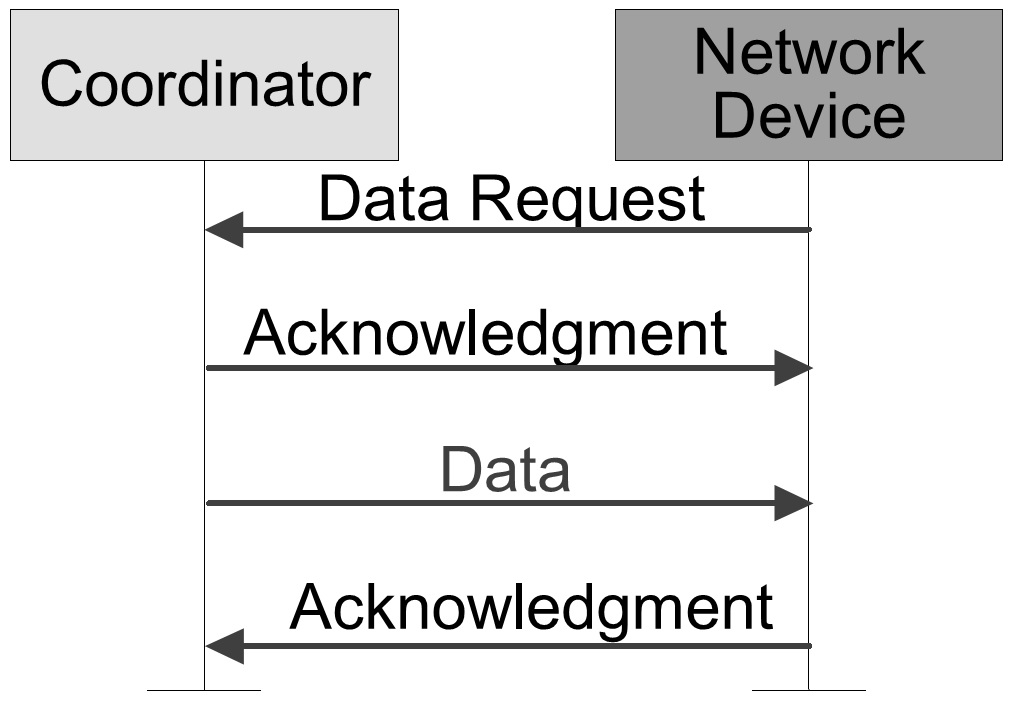
\includegraphics[height=.5\textheight]{./imagenes/coord-dev-sinbeacon.jpg}
                \vfill
                \caption{Coordinator $\rightarrow$ Device}
            \end{figure}            
        \end{minipage}
    \end{column}
\end{columns}          
\end{frame}


%-------------------------------------------------%
\subsection[Peer-to-Peer]{Topología Peer-to-Peer}
%-------------------------------------------------%
\begin{frame}[t]{Ejercicio 2: Topología Peer-to-Peer}{Comunicación sencilla}
    \begin{itemize}
        \item Agruparse en 2 grupos de 2 Mote cada uno.
        \vspace{5px}
        \item Los grupos se llamarán: PAN ID 1 y PAN ID 2.
        \vspace{5px}
        \item Cada PAN esta formada por: 1 coordinador y 1 device.
        \vspace{5px}
        \item Transferencia de datos:
            \begin{itemize}
            \item Sin beacon.
            \vspace{5px}
            \item La inicia el device.
            \vspace{5px}   
            \item Encender un led al transmitir y otro al recibir una trama.
            \vspace{5px}
            \end{itemize}
        \item La recepción de una trama es bloqueante.
        \vspace{5px}
    \end{itemize}
\end{frame}

%-------------------------------------------------%
\subsection[P2P+Verificar]{P2P + Verificar trama}
%-------------------------------------------------%
\begin{frame}[t]{Ejercicio 3: P2P + Verificación de trama}{Comunicación sencilla con verificación de trama}
    \begin{itemize}
        \item Partiendo de la comunicación establecida en el Ejercicio 2, verificar el contenido de la trama recibida:
        \vspace{5px}
            \begin{itemize}
            \item Verificar direccionamiento: La dirección de destino debe ser la dirección local.
            \vspace{5px}
            \item Verificar payload: El payload contiene un mensaje acordado por cada grupo.
            \vspace{5px}
            \end{itemize}
        \vspace{5px}
    \end{itemize}   
\end{frame}

%-------------------------------------------------%
\subsection[Inter PAN]{Inter PAN}
%-------------------------------------------------%
\begin{frame}[t]{Ejercicio 4: Inter PAN}{Comunicación entre dispositivos de distintas PAN}
    \begin{itemize}
        \item Transferencia de datos:
            \begin{itemize}
            \item Sin beacon.
            \vspace{5px}
            \item La inicia el device de la PAN ID 1.
            \vspace{5px}   
            \item La trama se envía al device de la PAN ID 2.
            \vspace{5px}
            \item La comunicación entre dispositivos de distintas PAN se hace a través de los coordinadores.
            \vspace{5px}
            \end{itemize}
        \item Verificar el contenido de la trama recibida.
        \vspace{5px}
            \begin{itemize}
            \item Verificar direccionamiento: La dirección de destino debe ser la dirección local.
            \vspace{5px}
            \item Verificar payload: El payload contiene un mensaje acordado por ambos grupos.
            \vspace{5px}
            \end{itemize}
        \vspace{5px}
    \end{itemize}   
\end{frame}

%-------------------------------------------------%
%-------------------------------------------------%
\section{Referencias}
%-------------------------------------------------%
%-------------------------------------------------%

\begin{frame}[c]{Referencias}

%\Large{Referencias}
\vspace{20px}
\begin{itemize}
	\item<.-> \href{http://ecee.colorado.edu/~liue/teaching/comm_standards/2015S_zigbee/802.15.4-2011.pdf}{Estándar IEEE 802.15.4:2011}
	\vspace{5px}	
	\item<.-> \href{http://www.ieee802.org/15/pub/TG4.html}{IEEE 802.15 - Task Group 4 - Home Page}
	\vspace{5px}
	\item<.-> \href{	https://standards.ieee.org/about/get/802/802.15.html}{IEEE Get Program}
	\vspace{5px}
	\item<.-> \href{http://www.nxp.com/documents/data_sheet/LPC1311_13_42_43.pdf}{LPC1343 - Datasheet}
	\vspace{5px}
	\item<.-> \href{http://www.nxp.com/documents/user_manual/UM10375.pdf}{LPC1343 - User Manual}
	\vspace{5px}
	\item<.-> \href{http://www.ti.com/product/CC2520/technicaldocuments}{Texas Instrument CC2520 -  Technical Documents}
	\vspace{5px}
	\item<.-> \href{http://www.ti.com/lit/an/swru120b/swru120b.pdf}{Texas Instrument Design Note - 2.4 GHz Inverted F Antenna}
\end{itemize}
\end{frame}

%\section*{cartón de gracias}

\begingroup
\makeatletter
\setlength{\hoffset}{-.5\beamer@sidebarwidth}
\makeatother
\begin{frame}[plain,noframenumbering]
\begin{center}
%\vspace{5px}
\hfill
    \begin{beamercolorbox}[center,dp=3ex,ht=10.25ex, wd=1\linewidth]{bgcolor}
        \Large\textbf{Protocolos de Comunicación en Sistemas Embebidos}\\
        \huge\textbf{Práctica 802.15.4 LR-WPAN}
    \end{beamercolorbox}
\hfill\hfill
\\
\vspace{5px}
\textbf{Carrera de Especialización en Sistemas Embebidos - FIUBA}\\
\vspace{10px}
\texttt{Ing. Patricio Bos: pbos@fi.uba.ar}\\
\texttt{Esp. Ing. Juan Montilla: juanvmontillac@gmail.com}\\

\vspace{10px}

\begin{figure}[H]
	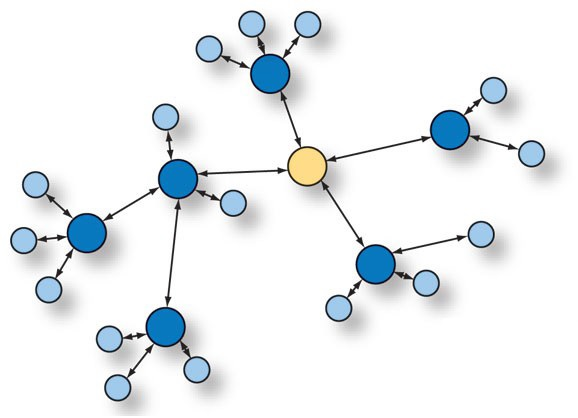
\includegraphics[width=.3\textwidth]{./imagenes/red.jpg}
\end{figure}	

\vspace{5px}
\tiny versión: 2016-06-06 rev 1.0 
 	  	
\end{center}
\end{frame}
\endgroup

\end{document}
